\documentclass{article}

\usepackage{amsmath}
\usepackage{graphicx}
\graphicspath{{images/}}

\setcounter{secnumdepth}{0}
\setlength{\parindent}{0pt}

\newcommand{\RP}{RP\vspace{0.1cm}\hrule\vspace{0.2cm}}
\newcommand{\SN}{SN\vspace{0.1cm}\hrule\vspace{0.2cm}}

\begin{document}

\section{Jan 8, 2022}
\RP
The github repo has been set up, and we have a function for identifying
non-collocation finite element points.

\vspace{0.5cm}\hrule\vspace{0.5cm}

Our next steps are to:
\begin{enumerate}
  \item Identify non-continuity, non-discretization constraints at
    non-collocation finite element points.
    These can be deactivated with \texttt{TemporarySubsystemManager}
    and solved as normal. The input, algebraic, and derivative variables
    at these points should not be included in the solve, which should
    lead to a non-degenerate KKT matrix.
    This is probably something we should check. We can't just check degeneracy
    of the equality Jacobian as it will be rectangular.

    (TODO: Should we deactivate other ``time-linking constraints'', such as
    those involving an integral, like a PI control law? -- yes, I believe
    these constraints should still be deactivated.)
  \item Invalidate input, algebraic, and derivative variables that were
    not sent to the solver (set values to None). How to identify these
    variables? Everything except differential variables? Or should we
    actually look for variables that don't appear in any constraints/objective
    that were sent to the solver? Ideally these are the same. Under what
    assumptions?
  \item Validate assumption: input, algebraic, and derivative variables
    at non-collocation finite element points don't appear other than in the
    constraints we deactivate. The first step here is to identify these
    variables. Then we can check that they don't appear in active constraints.
  \item These variables can then be plotted at points where they are
    valid (collocation points).
  \item A stretch goal would be to:
    \begin{enumerate}
      \item For some ``sufficient subset'' of input and algebraic variables
	(may have to be specified by user -- probably not unique),
	add constraints that specify these variables, likely by some
	interpolation.
      \item Assemble each system of equations (at each non-colloc FE point)
	that was deactivated (due to degeneracy), along with the new constraints
	to specify these systems, and solve each individually as a square
	system.
    \end{enumerate}
\end{enumerate}
This is a lot to code. It will be imporant to have a very clear motivation
for each addition.

\vspace{0.5cm}\hrule\vspace{0.5cm}

Reviewing Sakshi's code\dots

Works! Input variables at non-collocation finite element points are excluded
from the plotted control profile, because they have values of None, because
they were not sent to the solver, because the constraints they appear in
have been deactivated.
A couple directions we can go from here:
\begin{itemize}
  \item Start writing tests for functions we have so far. Get them
    ``PR-ready''
  \item In this example, ``wrong'' values are plotted if the inputs are
    initialized, say to $-1$. We could identify variables that were not
    sent to the solver, validate that they were not sent to the solver
    (don't appear in active constraints or objective), ``invalidate'' them
    (by setting them to None), and make sure we don't plot their values.
\end{itemize}

\section{Dec 22, 2021}
\RP
I have an approach I think will work for Radau collocation.
\begin{enumerate}
  \item Perform Dulmage-Mendelsohn
  \item Remove the square subsystem
  \item identify connected components
\end{enumerate}
Of course, there is a completely different approach that will work
for Radau and Legendre collocation, which is to just manually remove
(deactivate) all time-indexed constraints at non-collocation finite
element points.
The steps to do this are:
\begin{enumerate}
  \item Identify all time-indexed constraints
  \item At each finite element point that is not a collocation point
    (how to identify?), deactivate the constraint
\end{enumerate}
Will this leave us with a square model? What if an algebraic variable or
input at a non-collocation finite element point is used elsewhere in the
model (like an inequality constraint or the objective)?

\medskip

To actually make some progress implementing and testing these ideas, I should
set up a github repo that we can both work in.
I have set up the github repo and created a \texttt{dae\_testing} package.
What is the first thing I want to test? A function to get non-discretization,
non-continuity constraints at a particular point in time.

\medskip
Concrete tasks:
\begin{enumerate}
  \item For radau collocation, write function that correctly identifies
    non-discretization, non-continuity, equations (constraints) at
    non-collocation finite element points (which we happen to know is just
    $t=0$).
  \item Write the same function that works for Legendre discretziation.
  \item Test both of these on the homework example.
  \item Test them on CSTR example
\end{enumerate}

\section{Dec 21, 2021}

Sakshi's code runs. First thing I should do is parameterize the script
by discretization scheme. Have now done this, and I can generate plots with
radau and legendre discretizations and compare side-by-side.

\begin{figure}[!h]
  \centering
  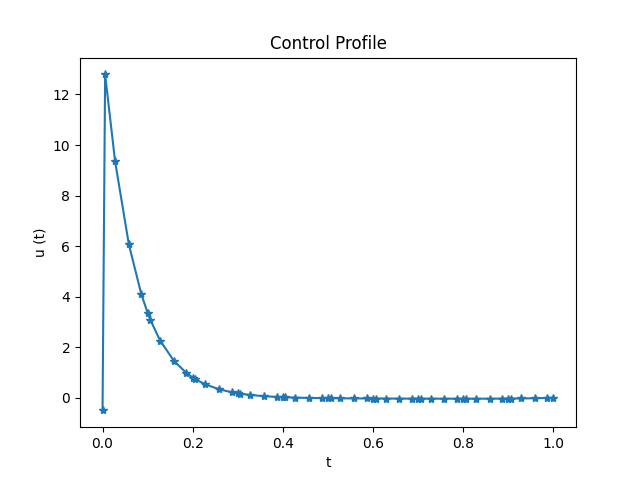
\includegraphics[width=5cm]{radau_control_profile.png}
  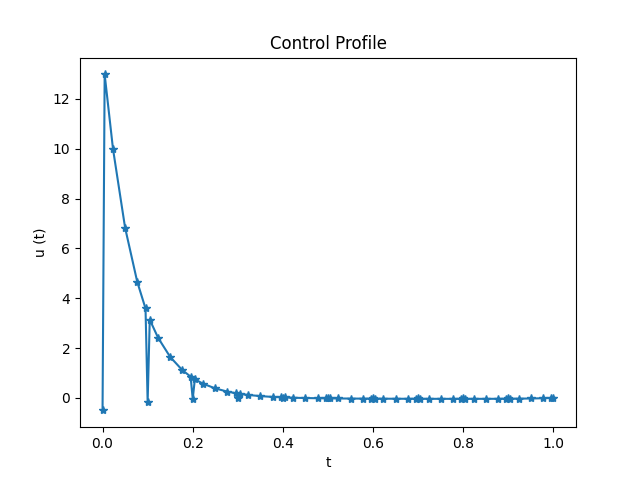
\includegraphics[width=5cm]{legendre_control_profile.png}
  \caption{Radau discretization, then legendre discretization}
\end{figure}

I suspect that the control variables are becoming arbitrary because they:
\begin{enumerate}
  \item Are free
  \item Have no effect on other variables
  \item Have no effect on the objective value
\end{enumerate}
How can I make this precise? First, I need to know which variables are my
inputs\ldots Just $u$ -- $x1$, $x2$, and $x3$ are states.
What is the path $u$ takes to influence the rest of the model, and why might
it be arbitrary here?

\[
u \rightarrow \frac{dx_1}{dt}, \frac{dx_2}{dt}, \frac{dx_3}{dt}
\rightarrow x_1, x_2, x_3 \text{ only at collocation points?}
\]

Things I'd like to check:
\begin{enumerate}
  \item What are all the variables ``influenced'' by $u$?
  \item Are there ``subsystems'' of model variables and equations that can
    be solved independently?
\end{enumerate}
What does Larry want us to answer?
\emph{Which variables can have arbitrary values?}
We suspect these are the control variables at non-collocation finite elements
points.
What is a sufficient condition for a variable to take an arbitrary value
during an optimization solve?
\begin{enumerate}
  \item It does not impact the value of the objective
  \item It is not part of a square subsystem\ldots, i.e. is not calculated
    by equality constraints.
\end{enumerate}
This is a bit tricky, as the variable value could be restricted by inequality
constraints.
How can I test if a variable influences the value of the objective?
If the variable ``influences the value'' of any of the variables in the
objective.
Given a matching and a DAG of variable calculation order, we can find the
variables necessary to calculate that one\ldots
This is more difficult in an optimization problem.

\end{document}
